\chapter{Einbinden von Grafiken und Sourcecode}
\label{Kap2}

\section{Bilder}

Natürlich können auch Grafiken und Bilder eingebunden werden, siehe z.\,B. Abbildung~\ref{Kap2:NasaRover}.

\begin{figure}[h]
  \centering
  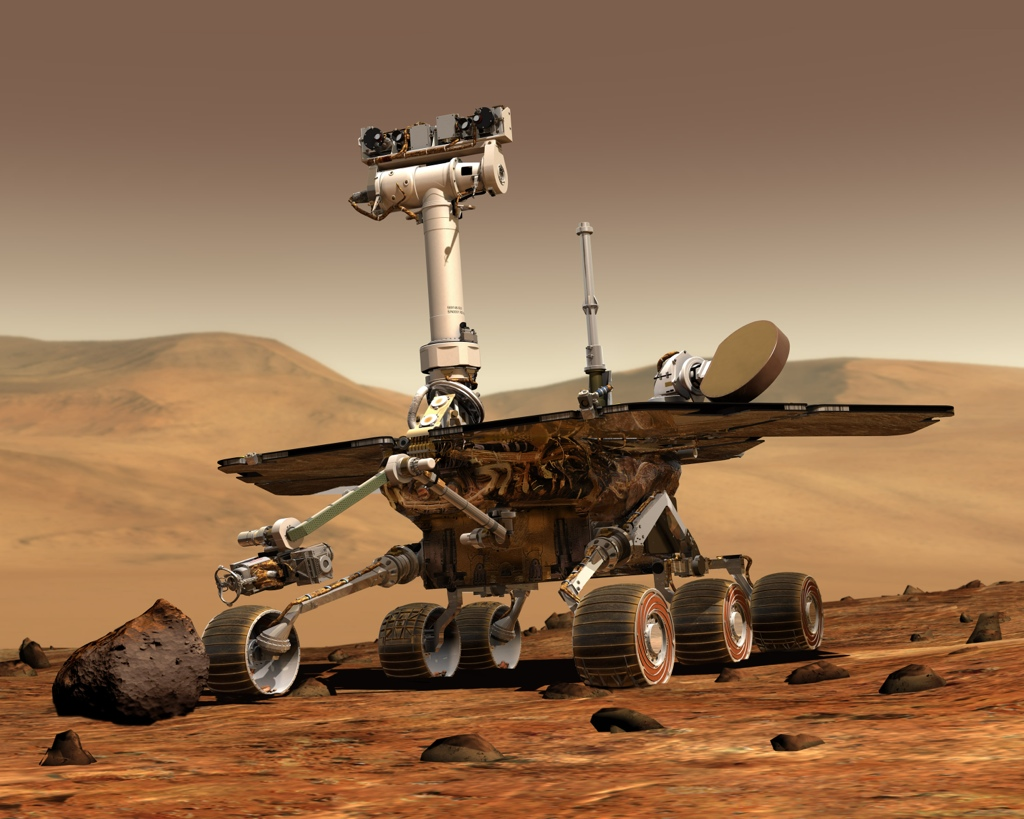
\includegraphics[width=6cm]{kapitel2/nasa_rover}
  \caption{Ein Nasa Rover}
  \label{Kap2:NasaRover}
\end{figure}


Man kann sich auch selber ein Makro für das Einfügen von Bildern schreiben:

\bild{kapitel2/modell_point_to_point}{6cm}{Point to Point}


\clearpage % Alle Bilder, die bisher kamen ausgeben



\section{Formelsatz}

Eine Formel gefällig? Mitten im Text $a_2 = \sqrt{x^3}$ oder als eigener Absatz (siehe Formel~\ref{Formel}):

\begin{equation}
\begin{bmatrix}         
   1 &  4 &  2 \\
   4 &  0 & -3 
\end{bmatrix}        
        \cdot
\begin{bmatrix}                
   1 &  1 &  0 \\
  -2 &  3 &  5 \\
   0 &  1 &  4 
\end{bmatrix}        
       {=} 
\begin{bmatrix}               
  -7 &  15 &  28 \\
   4 &   1 & -12 
\end{bmatrix}
\label{Formel}
\end{equation}


\section{Sourcecode}

Man kann mit Latex auch ganz toll Sourcecode in den Text aufnehmen.

\subsection{Aus einer Datei}

\lstinputlisting[firstline=2,language=Java,caption={Crypter-Interface},label=lst:CrypterInterface]{\srcloc/Crypter.java}


\subsection{Inline}

\begin{lstlisting}[language=Java,caption=Methode checkKey()]
    /**
     * Testet den Schlüssel auf Korrektheit: Er muss mindestens die Länge 1
     * haben und darf nur Zeichen von A-Z enthalten.
     *
     * @param key zu testender Schlüssel
     * @throws CrypterException wenn der Schlüssel nicht OK ist.
     */
    protected void checkKey(Key key) throws CrypterException {

        // Passt die Länge?
        if (key.getKey().length == 0) {
            throw new CrypterException("Der Schlüssel muss mindestens " +
                    "ein Zeichen lang sein");
        }

        checkCharacters(key.getKey(), ALPHABET);
    }
\end{lstlisting}

